%% LyX 2.3.3 created this file.  For more info, see http://www.lyx.org/.
%% Do not edit unless you really know what you are doing.
\documentclass[twocolumn,english]{article}
\usepackage[T1]{fontenc}
\usepackage[latin9]{inputenc}
\usepackage{color}
\usepackage{babel}
\usepackage{float}
\usepackage{amsmath}
\usepackage{amssymb}
\usepackage{graphicx}
\usepackage[unicode=true]
 {hyperref}

\makeatletter
%%%%%%%%%%%%%%%%%%%%%%%%%%%%%% User specified LaTeX commands.
\usepackage{algorithm,algpseudocode}

\makeatother

\usepackage[style=numeric]{biblatex}
\addbibresource{project.bib}
\begin{document}
\title{Motion Planning for Autonomous Driving}
\author{Philippe Weingertner, Minnie Ho}
\maketitle

\section{Introduction}

\section{Related Work}

There is a rich litterature related to Motion Planning and a very
detailed survey is provided in \cite{7490340}. Among the first 4
successful participants of DARPA Urban Challenge in 2007, the approaches
vary but they fundamentally rely on a graph search where nodes correspond
to a configuration state and edges correspond to elementary motion
primitives. The runtime and state space can grow exponentially large.
In this context, the use of efficient heuristic is important.

More recently, Reinforcement Learning and Deep RL have been investigated
in the context of Autonomous Driving for Decision Making either at
the Behavioural Planning or Motion Planning level. In papers from
Volvo \cite{DBLP:journals/corr/abs-1803-10056} and BMW \cite{inproceedings},
a DQN RL agent is trained to take decision at a tactical level: selecting
maneuvers. But the problem with Reinforcement Learning is that a utility
is optimized in expectation. So even if this utility is designed to
avoid collisions, this will be optimized in expectation only. In \cite{inproceedings}
an additional safety check layer is added after the DQN agent to eventually
override the DQN agent decision. In \cite{DBLP:journals/corr/abs-1904-07189}
RL is applied in the local planner: the action space is a set of longitudinal
accelerations applied along a given path at a T-intersection. The
agent is constrained to choose among a restricted set of safe actions
per state. So the safety is enforce before Deep RL. Ultimately we
may want combine both types of safety checks before and after an RL
agent.

In gaming, AlphaGo Zero \cite{Silver2017MasteringTG} has defeated
human world champions: thanks to a combination of MCTS tree search
and learning with Deep RL. A neural network biases the sampling towards
the most relevant parts of the search tree: a learnt policy-value
function is used as a heuristic during inference. There are a few
differences for Motion Planning. The state space is continuous, not
discrete, and only partially observable. Also self-play can not be
used. These challenges have been recently tackled in different publications.
The applicability of AlphaGo Zero ideas to Autonomous Driving has
been studied in \cite{DBLP:journals/corr/abs-1905-02680,DBLP:journals/corr/abs-1905-12197,8814125}.
In \cite{8814125} the Motion Planning problem is addressed in a 2
steps path-velocity decomposition. The path planner employs hybrid
A{*} to propose paths that are driveable and collision free wrt static
obstacles. In a second step a velocity profile is generated by issuing
acceleration commands. The problem is formulated as a POMDP model
and solved with an online DESPOT solver. DESPOT is a sampling based
tree search algorithm like MCTS which uses additional lower bounds
and upper bounds values. To guide the tree search of DESPOT, a NavA3C
neural network is used. The NavA3C network is trained in simulation
and is expected to provide tighter bounds. In \cite{DBLP:journals/corr/abs-1905-02680}
the problem is considered at the behavioral planning level. A set
of lane changes decisions are taken to navigate a highway and to reach
an exit. The problem is formulated as a MDP problem. MCTS tree search
is used as an online MDP solver and a learned policy-value network
is used to efficiently guide the search. 

We consider the problem of the local planner and velocity profile
generation, similar to the first paper, but with an approach mainly
aligned with the later one.

\section{Test Setup}

The problem statement is as follows. Given an ego vehicle (E) with
a given path of $(x,y)$ coordinates, find a set of acceleration decisions
$(a_{x},a_{y})$ at discrete time steps to enable E to avoid a set
of intersecting vehicles $\left\{ V\right\} .$

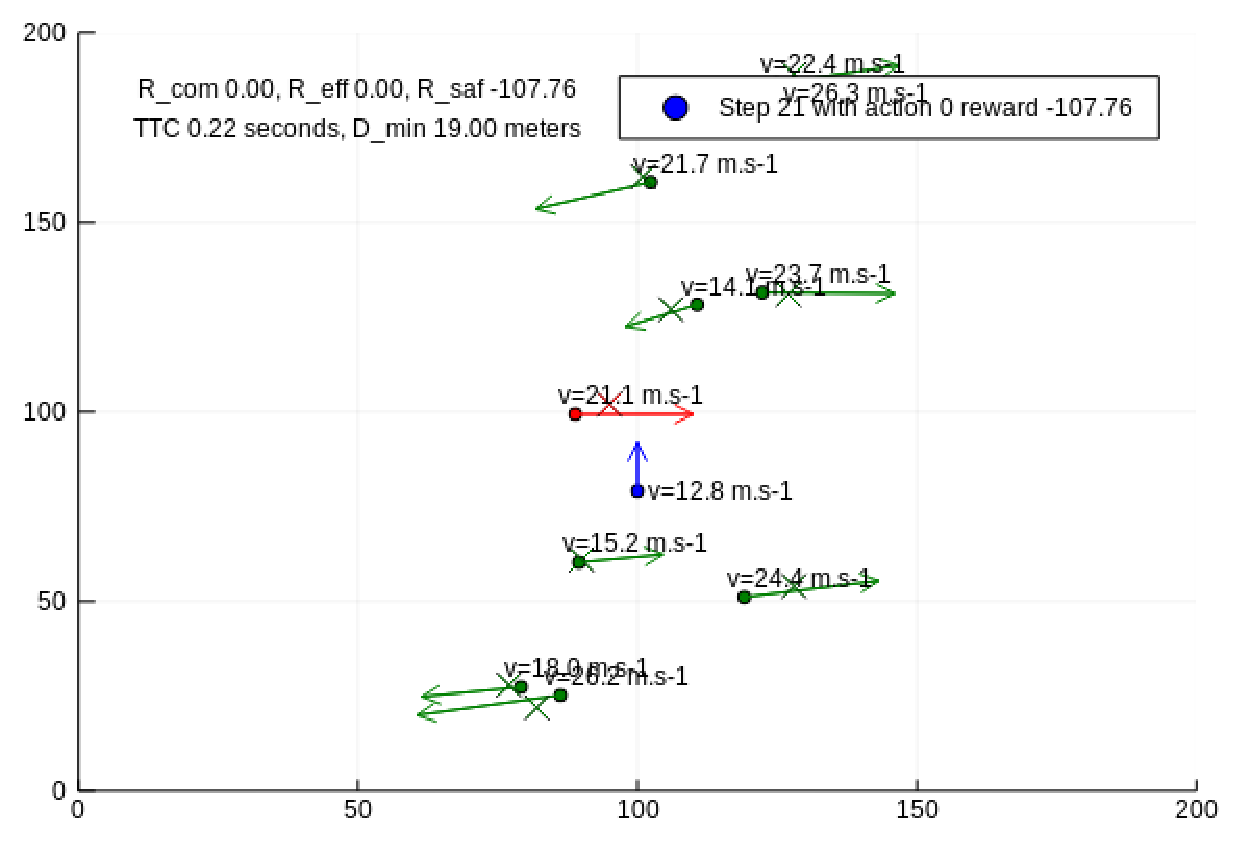
\includegraphics[scale=0.25]{img/ActV0}

The ego car in blue has to avoid 10 intersecting vehicles to reach
a goal point. The position and speed of intersecting vehicles is not
known precisely: the ground truth is represented via dots while the
position reported by the sensors is represented by crosses. A Time
To Collision based on ground truth information is displayed and if
there exists an intersecting car with a computed TTC below 10 seconds
it is displayed in red. We developped our own test framework but made
it compatible with \href{http://gym.openai.com/}{standard openai gym interfaces}.
Our simulation and test environment can be downloaded and installed
from \href{https://github.com/PhilippeW83440/CS221_Project/tree/master/gym-act}{gym-act}.

\section{Approach}

We are dealing with a local planning task where a path to follow has
been derived by some other algorithms (a variational technique or
some A{*} or D{*} tree search algorithm). We have to derive a set
of acceleration commands, such that we avoid dynamical obstacles that
may cross our path. We handle a sequential decision making problem
under uncertainty: the sensors provide noisy estimates. We first use
a model based approach (an online MCTS tree search algorithm). We
benchmark it against a model free approach (Q-learning or DQN). We
then combine the 2 approaches, to guide the MCTS tree search with
a learned heuristic. We target a fast, safe and explainable solution
as required for Autonomous Driving. We expect the safety and explainability
to be obtained thanks to the model based approach and to gain some
speed-up by using a model free learned heuristic.

\subsection{MDP model}

A representation of the states, position and speed information, in
absolute coordinates would be $S_{t}=\left\{ \left(x,y,v_{x},v_{y}\right)_{\text{ego}},\left(x,y,v_{x},v_{y}\right)_{\text{obj}_{1..10}}\right\} $.
But we use a relative and normalized representation for easier generalization
and learning. In our setting the ego car drives along the y-axis only\textbf{. }
\begin{itemize}
\item \textbf{States:} $S=\left\{ \left(\frac{y}{y^{max}},\frac{v_{y}}{v_{y}^{max}}\right)_{\text{ego}},\left(\frac{\Delta x}{\Delta x^{max}},\frac{\Delta y}{\Delta y^{max}},\frac{\Delta v_{x}}{\Delta v_{x}^{max}},\frac{\Delta v_{y}}{\Delta v_{y}^{max}}\right)_{\text{obj}_{1..10}}\right\} $
which is a vector $\in\mathbb{R}^{42}$ 
\end{itemize}
While the state space is continuous we use a discrete action space. 
\begin{itemize}
\item \textbf{Actions:} $A=\left[-2\;ms^{-2},-1\;ms^{-2},0\;ms^{-2},1\;ms^{-2},2\;ms^{-2}\right]$
corresponding to the longitudinal acceleration.\textbf{ }
\end{itemize}
The Transition model corresponds to standard linear Gaussian dynamics
with:
\begin{itemize}
\item \textbf{Transitions:} $T\left(s'\mid s,a\right)\text{ for each car}_{i}\;P\left(S_{i}^{t+1}\mid S_{i}^{t},a_{i}^{t}\right)=\mathcal{N}\left(\mu=T_{s}S_{i}^{t}+T_{a}a_{i}^{t},\Sigma\right)$ 
\end{itemize}
Using a Constant Velocity Model with $T_{s}=\begin{bmatrix}1 & 0 & \text{dt} & 0\\
0 & 1 & 0 & \text{dt}\\
0 & 0 & 1 & 0\\
0 & 0 & 0 & 1
\end{bmatrix},S_{i}^{t+1}=\begin{bmatrix}x\\
y\\
v_{x}\\
v_{y}
\end{bmatrix},T_{a}=\begin{bmatrix}\frac{\text{dt}^{2}}{2} & 0\\
0 & \frac{\text{dt}^{2}}{2}\\
\text{dt} & 0\\
0 & \text{dt}
\end{bmatrix},a_{i}^{t}=\begin{bmatrix}a_{x}\\
a_{y}
\end{bmatrix}$. The reward model accounts for efficiency (we penalize every step),
safety (we heavily pernalize collisions) and comfort (we penalize
strong accelerations and decelerations:
\begin{itemize}
\item \textbf{Reward}: $R(s,a)=-1-1000\times1\left[\text{d(ego,obj)}_{s}\leq10\right]-1\left[\left|a\right|=2\right]$
\end{itemize}

\subsection{Algo 1, MCTS tree search}

The MDP is solved online with MCTS tree search. Solving it offline
with Value Iteration is not an option as we are dealing with a huge
state space. MCTS \cite{Kochenderfer2015} is one of the most successfull
sampling-based online approaches used in recent years. It is the core
part of AlphaGo Zero \cite{DBLP:journals/corr/abs-1712-01815}. This
algorithm involves running many simulations from the current state
while updating an estimate of the state-action value function $Q(s,a)$
along its path of exploration. Online algorithms enable to reduce
the search space to reachable states from a current state. MCTS balances
exploration and exploitation via a method called Upper Confidence
Bound: during the search we execute the action that maximizes $Q(s,a)+c\sqrt{\frac{\log N(s)}{N(s,a)}}$
where $N(s),N(s,a)$ track the number of times a state and state-action
pair are visited. $c$ is a parameter controlling the amount of exploration
in the search: it will encourage exploring less visited $(s,a)$ pairs
and rely on the learned policy via $Q(s,a)$ estimates for pairs that
are well explored. Once we reach a state that is not part of the explored
set, we iterate over all possible actions from that state and expand
the tree. After the expansion stage, a rollout is performed: it consists
in running many random simulations till we reach some depth. It is
a Monte Carlo estimate so the rollout policy is typically stochastic
and does not have to be close to optimal. The rollout policy is different
than the policy used for exploration. Simulations, running from the
root of the tree down to a leaf node expansion, followed by a rollout
evaluation phase, are run until some stopping criterion is met: a
time limit or a maximum number of iterations. We then execute the
action that maximizes $Q(s,a)$ at the root of the tree. The pseudo
code of the algorithm is provided below:

{\scriptsize{}\begin{algorithmic}[1] 
\Function{SelectAction}{$s,d$} 
	\Loop
		\State \Call {Simulate}{$s,d,\pi_0$}
	\EndLoop
	\State \Return arg max$_a\text{ }Q(s,a)$
\EndFunction
\end{algorithmic}}{\scriptsize\par}

{\scriptsize{}\begin{algorithmic}[1] 

\Function{Simulate}{$s,d,\pi_0$} 
	\If {$d=0$}
		\State \Return $0$
	\EndIf

	\If {$s \notin T$} 
		\For {$a \in A(s)$}
			\State $(N(s,a),Q(s,a)) \gets (N_0(s,a),Q_0(s,a))$
		\EndFor
		\State $T=T \cup \{s\}$
		\State \Return \Call {Rollout}{$s,d,\pi_0$} 
	\EndIf

	\State $a \gets \text{arg max}_a\text{ }Q(s,a)+c\sqrt{\frac{logN(s)}{N(s,a)}}$ 
	\State $(s',r) \sim G(s,a)$
	\State $q \gets r+\lambda$ \Call {Simulate}{$s,d-1,\pi_0$}
	\State $N(s,a) \gets N(s,a)+1$
	\State $Q(s,a) \gets Q(s,a)+ \frac{q-Q(s,a)}{N(s,a)}$
	\State \Return $q$ 
\EndFunction

\end{algorithmic}}{\scriptsize\par}

{\scriptsize{}\begin{algorithmic}[1] 

\Function{Rollout}{$s,d,\pi_0$} 
	\If {$d=0$}
		\State \Return $0$
	\EndIf
	\State $a \sim \pi_0(s)$
	\State $(s',r) \sim G(s,a)$
	\State \Return $r+\lambda$ \Call {Rollout}{$s',d-1,\pi_0$}
\EndFunction
\end{algorithmic}}{\scriptsize\par}

One remaining problem is that in chess or go, the state space is discrete
and the above algorithm does not cope with continuous state space:
the same state may never be sampled more than once from the generative
model which will result in a shallow tree with just one layer. The
Progressive Widening variant of MCTS \cite{DBLP:journals/corr/abs-1709-06196,Couetoux:2011:CUC:2177360.2177393}
solves this problem by controlling the sampling of new states and
the sampling among already existing states to enable exploration in
depth and not just in breadth. 

\subsection{Algo 2, Approximate Q-learning}

While similarly to \cite{Silver2017MasteringTG,DBLP:journals/corr/abs-1905-12197,DBLP:journals/corr/abs-1905-02680,DBLP:journals/corr/abs-1712-01815,8814125}
we intend to use Deep Learning to learn an evaluation function that
will be used later on as a heuristic to guide the MCTS tree search,
we will first investigate Approximate Q-learning with a reduced set
of features. Weuse the following features extractor. $\phi(s,a)=\begin{bmatrix}s_{6\times1} & a_{1\times1} & s_{6\times1}^{2} & a_{1\times1}^{2}\end{bmatrix}^{T}$
where we take into account the state vector of the ego car (2 components)
and the state vector of the car with the smallest TTC (4 components).
We also take into account the acceleration command of the ego car.
We use quadratic components as well: as it is expected that the value
of a $(s,a)$ tuple will depend on distances computations. We focus
on a reduced set of relevant features to speed up training. The Q-function
is parametrized by a vector $w$ with $\hat{Q}_{\text{opt}}(s,a;\mathbf{w})=\mathbf{w}\cdot\phi(s,a)$.
We have $\hat{V}_{\text{opt}}(s')=\underset{a'\in\text{Actions}(s')}{\max}\hat{Q}_{\text{opt}}(s',a')$
and use the objective $\left(\hat{Q}(s,a;\mathbf{w})_{\text{pred}}-{\color{green}{\normalcolor \left(r+\gamma\hat{V}_{\text{opt}}(s')\right)_{\text{targ}}}}\right)^{2}$
which leads to the following update rule while performing Sochastic
Gradient Descent: $\mathbf{w}\leftarrow\mathbf{w}-\eta\left[\hat{Q}_{\text{opt}}(s,a;\mathbf{w})_{\text{pred}}-{\color{green}{\normalcolor \left(r+\gamma\hat{V}_{\text{opt}}(s')\right)_{\text{targ}}}}\right]\phi(s,a)$.
One of the problem we may encounter is that the data in simulation
is not iid, but highly correlated from one simulation step to the
other and the targets will vary a lot. This problem is typically handled
by using an experience replay buffer, which is possible with an off
policy algorithm, and using a different fixed Q-network for targets
evaluation, which is updated less frequently than the Q-function used
for predictions, as described in DeepMind papers \cite{article,DBLP:journals/corr/MnihKSGAWR13}. 

\subsection{Algo 3, Deep Q-learning}

We use a DQN algorithm with a replay memory buffer to ensure we are
dealing with iid samples and a target network, updated less frequently
than the optimisation network, to stabilize the training procedure
as described in DeepMind papers \cite{article,DBLP:journals/corr/MnihKSGAWR13}.
We use a Huber Loss which acts as MSE when error is small and as a
mean absolute error when error is large: to make it more robust to
outliers when the estimates of $Q$ are very noisy. Exploration is
done with an $\epsilon$ -greedy policy. We use a batch size of $128$,
$\gamma=0.999$ and Adam optimizer for the Batch Gradient Descent
updates. Programming is done with pytorch and we leverage on this
code \href{https://pytorch.org/tutorials/intermediate/reinforcement_q_learning.html}{pytorch.org}
as a starting point for the DQN setup.

Our Neural Network has 42 neurons as input, corresponding to all cars
position and speed information (relative and normalized coordinates),
and 5 neurons as output, corresponding to the 5 possible control commands.
We use a Neural Network architecture slightly adapted from \cite{DBLP:journals/corr/abs-1803-10056},
based on a CNN network as we want translational invariance of the
input: it should not matter to provide information about different
cars in one order or the other.
\begin{center}
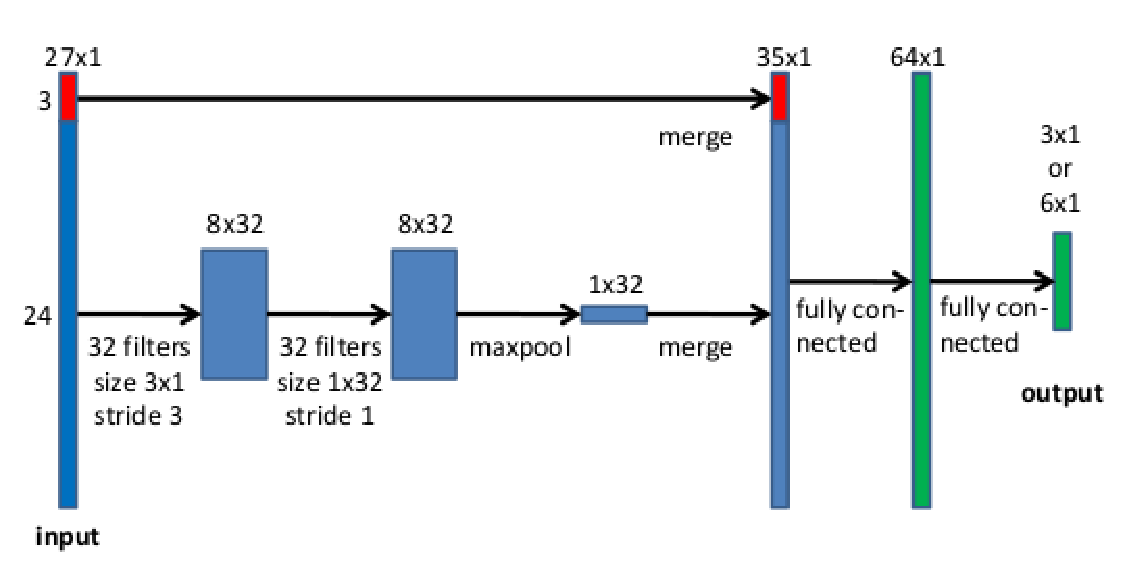
\includegraphics[scale=0.3]{img/CNN_for_DQN}
\par\end{center}

\subsection{Algo 4, MCTS tree search with a learned heuristic }

We plan to use our learned Q-network $\hat{Q}(s,a;\mathbf{w})$ via
approximate Q-learning or Deep Q-learning as a heuristic for MCTS
tree search: to expand the tree in the most promising areas and hence
come up faster with a good solution. A solution is considered good
as soon as it is estimated collision free. We are dealing with uncertainty
so it is an estimate. We may run further MCTS tree searches up to
some time limit, to find even better solutions: faster or more comfortable.

\section{Experiments}

The source code is available here: \href{https://github.com/PhilippeW83440/CS221_Project}{CS221 Project}.
The baseline (simple rule - reflex based) and oracle (assuming no
uncertainty using UCS/A{*} tree search) have been implemented at the
proposal stage. For the progress report, we have a first version of
Q-learning with some results summarized in the appendix. We are working
on the MCTS implementation.

\nocite{*}
\printbibliography

\end{document}
